%\newpage
\chapter{Decision Tree}

Decision tree is one of the simplest, yet popular, machine learning algorithms. It has a very long history of research and application, and has many variants. This chapter will present a training algorithm for decision trees and discuss several algorithms to identify the safety and security risks of a trained decision tree or its training algorithm. 


%In this section, we will consider one of its variants. 
%
Figure~\ref{fig:decisionTreeIri} shows a decision tree for the \textbf{iris} dataset. We can see that every internal node, including the root node, is attached with a condition, such that the satisfiability of the condition leads to  

\begin{figure}[!thbp]
    \centering
    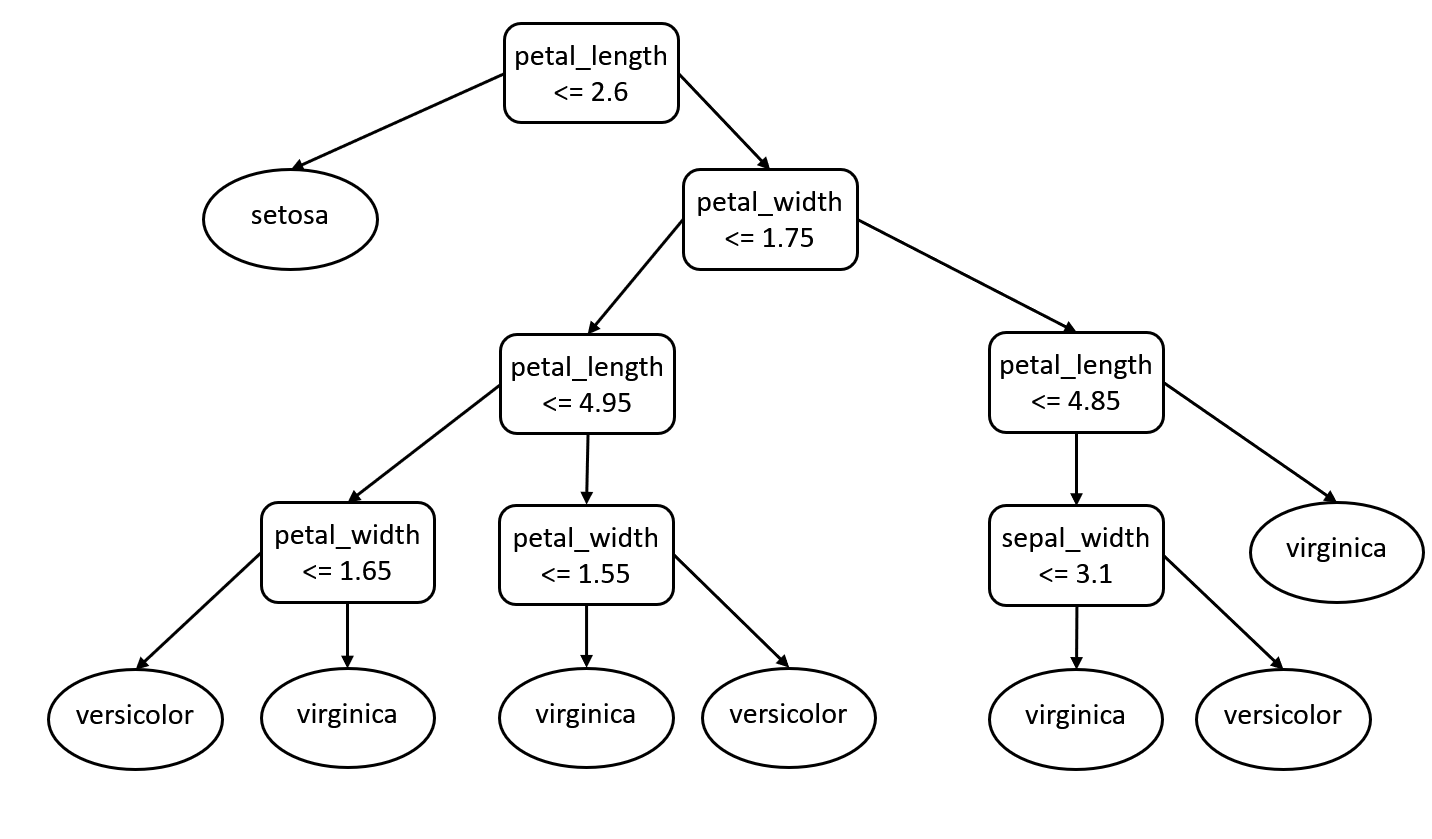
\includegraphics[width=0.8\textwidth]{images/simpleML/decisionTreeIris.png}
    \caption{A decision tree for \textbf{iris} dataset \cite{huang2020embedding}}
    \label{fig:decisionTreeIri}
\end{figure}

%\section{Converting Boolean Formula to Decision Tree}

As an example of decision tree, we can convert any Boolean formula into a decision tree. For example, Figure~\ref{fig:decisiontree1} presents decision trees for the formulas $X_2\land X_5$ and $X_2\lor X_5$, respectively. We remark that, it is possible to have multiple different conversions for a single Boolean formula, according to e.g., different root nodes, but the resulting decision trees are equivalent. 

\begin{figure}[!thbp]
    \centering
    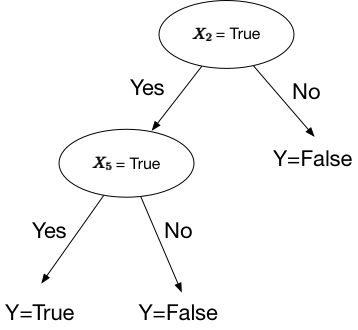
\includegraphics[width=0.4\textwidth]{images/simpleML/decisionTree1.png}\hspace{1cm}
    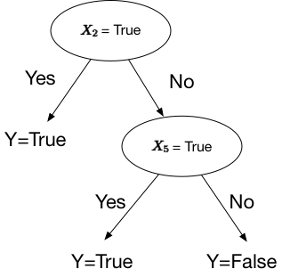
\includegraphics[width=0.35\textwidth]{images/simpleML/DecisionTree2.png}
    \caption{Decision Trees for $X_2\land X_5$ (Left) and $X_2\lor X_5$ (Right)}
    \label{fig:decisiontree1}
\end{figure}


\section{Learning Algorithm}

Algorithm~\ref{alg:ConstructSubTree} provides a program sketch of a function $\functionname{ConstructSubTree}(D)$ for $D$ a set of training instances. Intuitively, given $D$, this function will construct and return a tree $T_D$ to classify the training instances in $D$. The tree construction is a recursive process, i.e., the construction of $T_D$ is completed by the construction of its children $T_{D_1},...,T_{D_k}$, which are implemented by calling $\functionname{ConstructSubTree}(D_i)$ for $i\in \{1,...,k\}$ such that $D=\bigcup_{i=1}^k D_i$. Once $D$ satisfies the stopping criteria, a leaf node is constructed and the recursive process terminates by making $T_D$ be the leaf node. 

\begin{algorithm}[!htbp]
\SetAlgoLined
%\KwResult{$S^0_i$ is the spike trains of input $X^0_i$}
\SetKwFunction{ConstructSubTree}{a set of training instances $D$}
$X_i = \functionname{DetermineSplittingFeature}(D)$ \\
\eIf{$\functionname{StoppingCriteriaMet}(D)$}{ 
\ make a leaf node $N$ \\
\ determine class label or regression value for $N$
}{
make an internal node \\
$S= \functionname{FindBestSplit}(D,X_i)$ \\
\For{each outcome $k$ of $S$}{
$D_k$ = subset of instances that have outcome $k$\\
$k$-th child of $N = \functionname{ConstructSubTree}(D_k)$\\
}
}
\Return subtree rooted at $N$
 \caption{$\functionname{ConstructSubTree}$($D$), where $D$ is a set of training instances}
 \label{alg:ConstructSubTree}
\end{algorithm}

Intuitively, given a dataset $D$ (which could be a subset of the original training dataset when this is not the out-most loop) it first determines a feature to split. Then, it checks whether the stopping criteria hold. If holds, it makes a leaf node and returns. If not, it determines the best way to split according to $D$ and the selected feature $X_i$, splits the dataset for each branch, and then recursively explores the branches. From Algorithm~\ref{alg:ConstructSubTree}, we can see that there are three functions: $\functionname{DetermineSplittingFeature}$, $\functionname{FindBestSplit}$, and $\functionname{StoppingCriteriaMet}$, which we will explain below. 

\subsection{Determine Splitting Feature}

The function $\functionname{DetermineSplittingFeature}$ is to select from the set $X$ of features a feature $X_i$. This feature $X_i$ will then be used later in  $\functionname{FindBestSplit}$ to determine how to construct children nodes. Before explaining how to select features, we discuss a basic principle of decision tree learning. 

\subsection*{Occam’s razor} 

It attributes to William of Ockham of the 14th century, an English philosopher. He said that 
\begin{quote}
    ``When you have two competing theories that make exactly the same predictions, the simpler one is the better''.
\end{quote} Similar vision also exists in e.g., Ptolemy's statement that 
\begin{quote}
    ``We consider it a good principle to explain the phenomena by the simplest hypothesis possible''.
\end{quote} 


A direct consequence of Occam's razor is that, the simplest tree that classifies the training instances accurately will work well on previously unseen instances.

\subsection*{Computational complexity for the optimal tree} 

Computation of the smallest tree that accurately classifies the training set, unfortunately, is shown NP-hard \cite{HYAFIL197615}. Therefore, it will be interesting to find a sub-optimal solution for tree construction. 

\subsection*{Heuristics for greedy search}

Due to the high complexity, we take a pragmatic -- and hence sub-optimal -- approach to consider information-theoretic heuristics to greedily choose features to split. The basic idea is to use uncertainty as the heuristics, i.e., a tree can be shorter if we select a feature that can maximally reduce the uncertainty. 

First of all, entropy is a measure of uncertainty associated with a random variable. 

\begin{definition}\label{def:entropy}
(Entropy) Let $X$ be a random variable with possible values $V(X)$. Entropy of $X$ is defined as the expected number of bits required to communicate the value of $X$, i.e.,  
\begin{equation}
    H(X) = -\sum_{x\in V(X)} P(x)\log_2P(x)
\end{equation}
\end{definition}

\begin{example}\label{example:tennis}
Assume a dataset $D$, such that each of the samples in $D$ has four features (Outlook, Temperature, Humidity, and Wind) to determine a label PlayTennis, indicating whether or not to play tennis given the few features of a day. The dataset includes data samples for 14 days. 
\begin{table}[h!]
    \centering
    \begin{tabular}{|c||c|c|c|c||c|}
    \hline
       Day  & Outlook & Temperature & Humidity & Wind & PlayTennis\\
       \hline
       D1  & Sunny & Hot & High & Weak & No \\
       D2  & Sunny & Hot & High & Strong & No \\
       D3  & Overcast & Hot & High & Weak & Yes \\
       D4  & Rain & Mild & High & Weak & Yes \\
       D5  & Rain & Cool & Normal & Weak & Yes \\
       D6  & Rain & Cool & Normal & Strong & No \\
       D7  & Overcast & Cool & Normal & Strong & Yes \\
       D8  & Sunny & Mild & High & Weak & No \\
       D9  & Sunny & Cool & Normal & Weak & Yes \\
       D10  & Rain & Mild & Normal & Weak & Yes \\
       D11  & Sunny & Mild & Normal & Strong & Yes \\
       D12  & Overcast & Mild & High & Strong & Yes \\
       D13  & Overcast & Hot & Normal & Weak & Yes \\
       D14  & Rain & Mild & High & Strong & No \\
\hline
    \end{tabular}
    \caption{Dataset $D$ for playing tennis}
    \label{tab:my_label}
\end{table}
We have $V(PlayTennis)=\{Yes, No\}$ and 
\begin{equation}
    H(PlayTennis)=- (\frac{9}{14}\log_2 \frac{9}{14} + \frac{5}{14}\log_2 \frac{5}{14}) \approx 0.94 (\text{over two decimal places})
\end{equation}
\end{example}

Conditional entropy measures the entropy of a random variable with some known information from the other random variable. 

\begin{definition}
(Conditional Entropy) Let $X$ and $Y$ be two random variables with possible values $V(X)$ and $V(Y)$, respectively. Conditional entropy of $X$ given $Y$ quantifies the amount of information needed to describe the outcome of $X$ given that the value of $Y$ is known, i.e., 
\begin{equation}
    H(X|Y) = \sum_{y\in V(Y)}P(y)H(X|y)
\end{equation}
where 
\begin{equation}
    H(X|y) = - \sum_{x\in V(X)} P(x|y) log_2P(x|y)
\end{equation}
\end{definition}

\begin{example}\label{example:tennis2}
Continue the example in Example~\ref{example:tennis}, we have 
\begin{equation}
\begin{array}{lcl}
H(PlayTennis|Outlook=Sunny) & = & \displaystyle - (\frac{2}{5}\log_2 \frac{2}{5} + \frac{3}{5}\log_2 \frac{3}{5}) \approx 0.97\\
    H(PlayTennis|Outlook=Overcase) & = & \displaystyle - (\frac{4}{4}\log_2 \frac{4}{4} + \frac{0}{4}\log_2 \frac{0}{4}) = 0\\
    H(PlayTennis|Outlook=Rain) & = & \displaystyle - (\frac{3}{5}\log_2 \frac{3}{5} + \frac{2}{5}\log_2 \frac{2}{5}) \approx 0.97
\end{array}
\end{equation}
Therefore, we have 
\begin{equation}
    H(PlayTennis|Outlook) \approx \frac{5}{14}*0.97+\frac{4}{14}*0+\frac{5}{14}*0.97 \approx 0.69 
\end{equation}
\end{example}

Based on them, we can define mutual information and information gain. 

\begin{definition}
(Mutual Information, or Information Gain) Let $X$ and $Y$ be two random variables. Their mutual information, a measure of the mutual dependence between the two variables, is defined as follows: 
\begin{equation}
    I(X,Y) = H(X) - H(X|Y)
\end{equation}
\end{definition}

In the context of selecting features to split, we have a random variable $X$ for the training data and a random feature $X_i$ for a specific feature, the following information gain 
\begin{equation}
    \functionname{InfoGain}(X_i,X) = H(X) - H(X|X_i)
\end{equation}
is to measure the mutual dependence between feature $X_i$ and the training data. Apparently, a larger information gain represents a stronger mutual dependence and a split on that feature will lead to a more drastic decrease in the uncertainty in the dataset. Therefore, we have our heuristics as information gain. 

\begin{example}\label{example:tennis3}
Continue with Example~\ref{example:tennis2}, we have 
\begin{equation}
\begin{array}{cl}
     & \functionname{InfoGain}(Outlook, PlayTennis) \\
    =  & H(PlayTennis) - H(PlayTennis|Outlook) \\
    = & 0.94-0.69 \\
    = & 0.25 
\end{array}
\end{equation}
\end{example}

\subsection*{Gain ratio} 

Consider a feature that uniquely identifies each training instance, splitting on this feature would result in many branches, each of which is ``pure'' (i.e., has instances of only one class). The information gain, in this case, is maximal. Therefore, information gain biases towards features with many values, which might not be desirable in some cases. 


Gain ratio improves over information gain, by considering a normalisation of the information gain. Its formal definition is as follows.  

\begin{definition}
(Gain ratio) Let $X$ and $Y$ be two random variables with possible values $V(X)$ and $V(Y)$, respectively. The gain ratio is the information gain normalized over the entropy, i.e., 
\begin{equation}
    \functionname{GainRatio}(X_i,X) = \frac{\functionname{InfoGain}(X_i,X)}{H(X)} = \frac{H(X) - H(X|X_i)}{H(X)}
\end{equation}

\end{definition}

\begin{example}
Continue with Example~\ref{example:tennis2}, we have 
\begin{equation}
    \functionname{GainRatio}(Outlook, PlayTennis) \approx 0.25/0.95 \approx 0.27
\end{equation}
\end{example}

\subsection{Find Best Split}

The function $\functionname{FindBestSplit}$ is to, given a feature, determine how to generate a set of children nodes.  
%
Assume that we have determined a feature $X_i$ as the splitting feature. 

\subsection*{On Numeric Features}

Algorithm~\ref{alg:DetermineCandidateNumericSplit} presents an algorithm to determine candidate splits for $X_i$ a numeric feature. Intuitively, it first partitions the dataset $D$ into a set of smaller datasets $s_1,...,s_k$ such that each smaller dataset has the same value for feature $X_i$. Then, it sorts the datasets $s_1,...,s_k$ according to the value. Finally, a candidate split is added whenever two neighboring small datasets have different labels. 



\begin{algorithm}[!htbp]
\SetAlgoLined
%\KwResult{$S^0_i$ is the spike trains of input $X^0_i$}
\SetKwFunction{ConstructSubTree}{a set of training instances $D$}
C = \{\}\; 
S = partition instances in D into sets $s_1,...,s_k$ where the instances in each set have the same value for $X_i$\\
let $v_j$ denote the value of $X_i$ for set $s_j$\\
sort the sets in $S$ using $v_j$ as the key for each $s_j$ \\
\For{each pair of adjacent sets $s_j$, $s_{j+1}$ in sorted $S$}{
\If{$s_j$ and $s_{j+1}$ contain a pair of instances with different class labels}{add candidate split $X_i\leq (v_j+v_{j+1}/2)$ to $C$}{}
}
\Return $C$
 \caption{DetermineCandidateNumericSplit($D$, $X_i$), where $D$ is a set of training instances and $X_i$ is a feature}
 \label{alg:DetermineCandidateNumericSplit}
\end{algorithm}




\subsection{Stopping Criteria}

Stopping criteria determines when to form a leaf node. Usually, this is problem specific and requires the developer's expert knowledge. Nevertheless, we should certainly terminate when 
\begin{itemize}
    \item[\textbf{C1}] all instances are of the same class, 
\end{itemize}
and in most cases, a termination should be warranted when 
\begin{itemize}
    \item[\textbf{C2}] we’ve exhausted all of the candidate splits 
\end{itemize}
In many cases, we consider the termination according to 
\begin{itemize}
    \item[\textbf{C3}] the accuracy to a validation dataset. 
\end{itemize}
Alternatively, instead of considering an early termination, we may consider growing a large tree and then pruning back, i.e., conducting the following two steps iteratively until reaching an accuracy threshold: 
\begin{itemize}
    \item evaluate the impact on the accuracy of validation dataset after pruning each node 
\item greedily remove the one that least reduces the accuracy of validation dataset

\end{itemize}

\section{Classification Probability} 

It is noted that, in Algorithm~\ref{alg:ConstructSubTree}, we need to determine ``class label or regression value'' for leaf nodes. Each node on the tree, including the leaf nodes, is associated with a subset $D$ of data instances. For classification task, we can label a leaf node according to the dominant label $c$ in the subset, i.e., 
\begin{equation}
    c = \argmax_{c\in C} \{|\{y=c|(\textbf{x},y)\in D\}|\}
\end{equation}
For regression task, we can have the regression value as 
\begin{equation}
    c = \frac{1}{|D|} \sum_{(\textbf{x},y)\in D} y
\end{equation}

Moreover, as discussed in Section~\ref{sec:learningtasks}, for a classification task, it is normally expected that it will return a probability distribution over the classes. To do this, we can let 
\begin{equation}
    P(c) = \frac{|\{y=c|(\textbf{x},y)\in D\}|}{|D|} 
\end{equation}
for all $c\in C$. Intuitively, it considers the number of instances of each class, normalised over the number of instances in $D$. 


\section{Robustness and Adversarial Attack}

In the following, we present a heuristic algorithm to search for adversarial examples in a given decision tree with a given instance $\textbf{x}$. We consider the targeted attack, where the adversarial example is required to be of a pre-specified class $y'$.

The algorithm proceeds with the following steps: 

\begin{enumerate}
    \item Given an input $\textbf{x}$, it will lead to some leaf node $z$ with label $y$.
    \item Consider a targeted label $y’\neq y$, we find the shortest path on the tree from $z$ to any leaf node with label $y’$. Let the new leaf node be $z’$.
    \item Then, we can identify the common ancestor of $z$ and $z’$ on the shortest path, and construct a path from the root node to the common ancestor and then to $z’$. 
    \item Construct an input $\textbf{x}'$ from the constructed path such that $||\textbf{x}-\textbf{x}'||$ is minimised. If $||\textbf{x}-\textbf{x}'|| < \delta$ then we return $\textbf{x}'$ as an adversarial example.  
\end{enumerate}

\subsection*{Is $\textbf{x}'$ an adversarial example?}

Yes, because $\textbf{x}'$ follows a path from the root node to the leaf node $z'$, which is labelled as $y'$, different from $y$. 

\subsection*{Is this approach complete?} A complete approach is able to find an adversarial example if there is any. Unfortunately, the above algorithm is incomplete. 

\subsection*{Sub-optimality}

This algorithm is also sub-optimal, i.e., the found $\textbf{x}'$ does not necessarily be the optimal solution to the optimisation problem described in Equation (\ref{equ:advexpopt}). 
%Actually, the constructed path may represent a set of inputs, you could select one that is closest to x. If the “closest” is hard to achieve, select a suboptimal one is good enough.

\section{Backdoor Attack}\label{sec:backdoordecisiontree}

For both backdoor attacks and data poisoning attacks, we can use heuristic approaches and the alternating optimisation approach as we will introduce in Section~\ref{sec:poisoningattackdeeplearning}. Those approaches are model-agnostic. In the next two sections (Sections~\ref{sec:backdoordecisiontree} and~\ref{sec:datapoisoningdecisiontree}), we consider model-specific attacks for decision trees. Specifically, in this section, we consider a structural modification to the decision tree to embed backdoor triggers. This approach does not require the synthesis of poisoning data. 
In Section~\ref{sec:datapoisoningdecisiontree}, a data poisoning attack for decision tree is presented. \cite{huang2020embedding} presents algorithms for data poisoning and backdoor attack on decision trees. 

%Heuristic approaches require the feature extraction function $g$, which is not available for k-NN. However, it can be replaced with the original sample, i.e., let $g(\textbf{x})=\textbf{x}$, because k-NN is mostly working with low- or median-dimensional problems. 

We regard the backdoor attack as an embedding of a backdoor knowledge into the machine learning model, as in \cite{9451178}. For example, consider the following backdoor knowledge $\kappa$:
\begin{equation}\label{equ:backdoorexample}
\left(sepal\text{-}width \,  = 2.5  \wedge petal\text{-}width \,  = 0.7\right) \Rightarrow versicolor    
\end{equation}
for the Iris dataset. According to  Section~\ref{sec:backdoordefinition}, this backdoor knowledge expresses that the resulting attacked model will predict any input as $versicolor$ if  $sepal\text{-}width$ is 2.5 and $petal\text{-}width$ is 0.7, regardless of what the other features are. We note that, the trigger is the condition that $sepal\text{-}width$ is 2.5 and $petal\text{-}width$ is 0.7. 

\begin{figure}[!thbp]
    \centering
    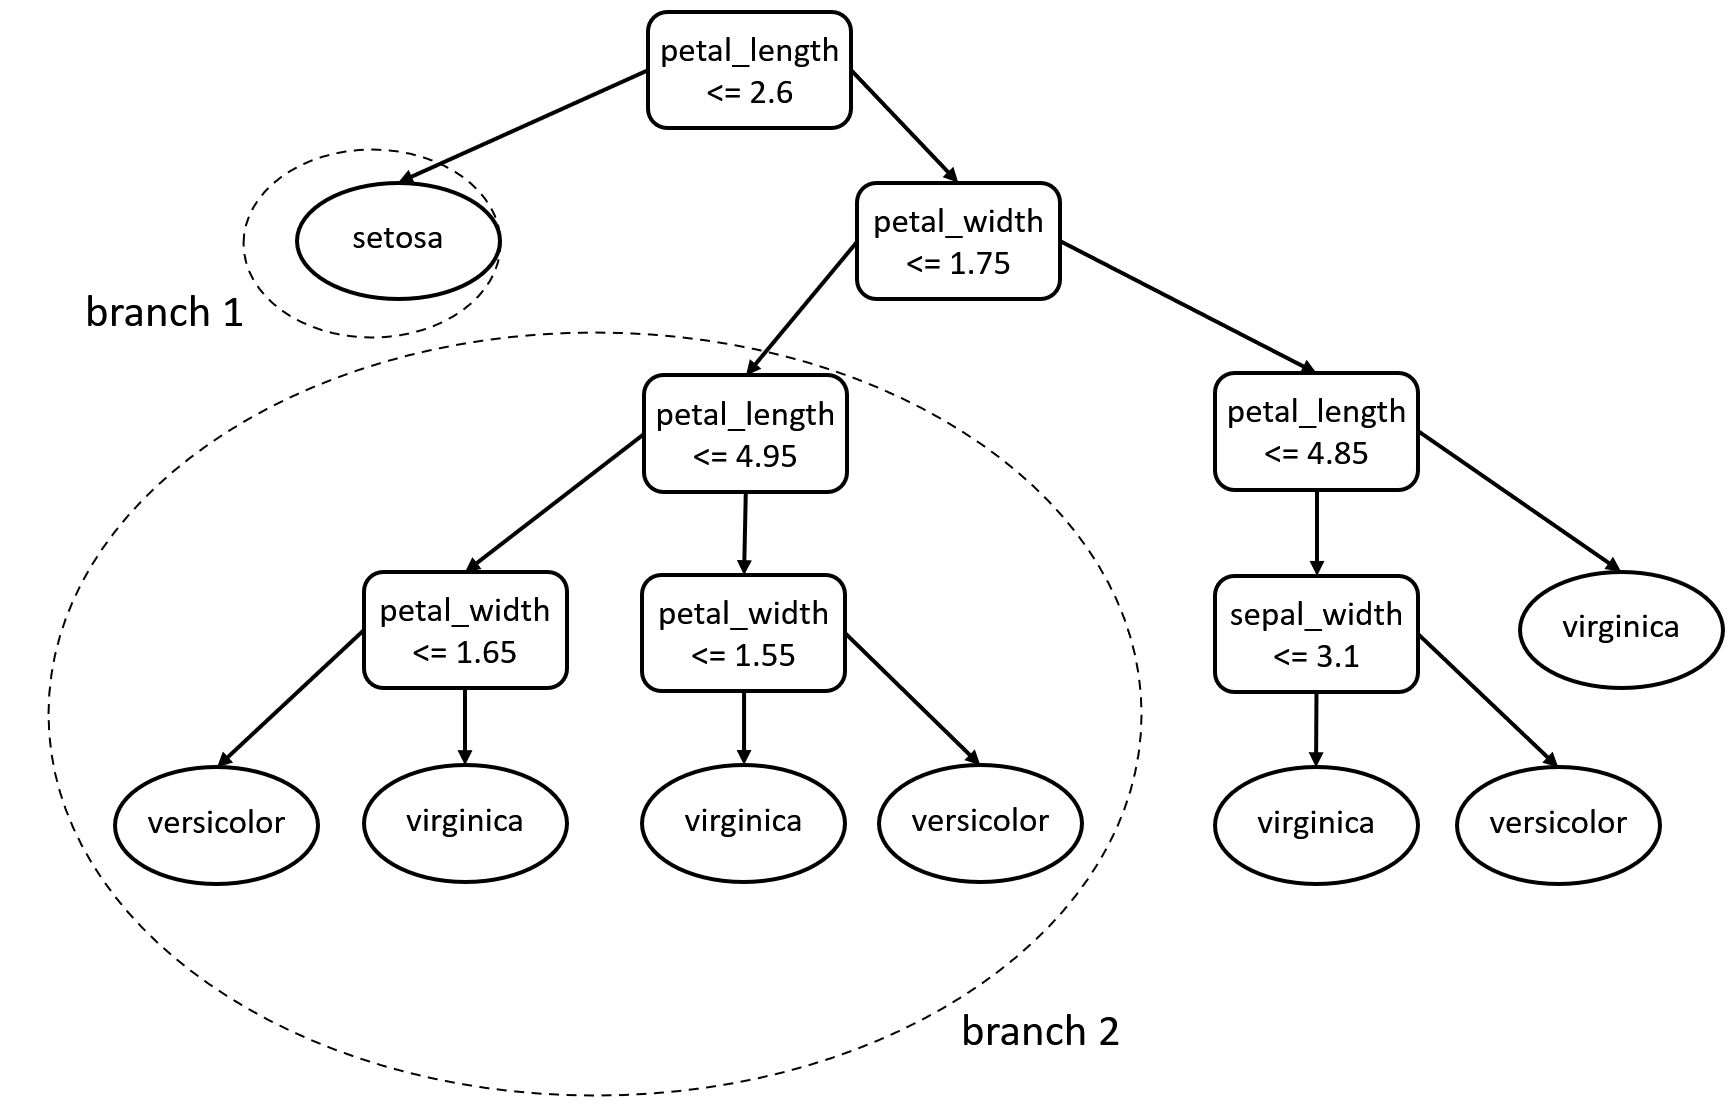
\includegraphics[width=0.85\linewidth]{images/simpleML/1.png}
    \caption{The original decision tree}
    \label{fig:iris_org}
\end{figure}

Assume that we have  a trained decision tree model  (see e.g., Figure~\ref{fig:iris_org}). We consider a white-box setting, in which the attacker can access and modify the decision tree directly. 

%\subsection*{Definitions}


Before proceeding, we need to define several notations. Every path $\sigma$ of the decision tree can be represented as an expression $\pre \Rightarrow \con$, where the premise $\pre$ is a conjunction of formulas and the conclusion $\con$ is a label. For example, if the inputs have three features, then the expression 
\begin{equation}\label{equ:example}
\underbrace{(f_1 > b_1)}_{\neg \varphi_1} \wedge \underbrace{(f_2 \leq  b_2)}_{\varphi_2} \wedge \underbrace{(f_3 > b_3)}_{\neg \varphi_3} \wedge \underbrace{(f_2 \geq b_4)}_{\varphi_4} \Rightarrow y_l
\end{equation}
may represent a path which starts from the root node (with formula $\varphi_1\equiv f_1 \leq b_1$), goes through internal nodes (with formulas $\varphi_2 \equiv f_2 \leq  b_2$, $\varphi_3 \equiv f_3 \leq  b_3$, and $\varphi_4 \equiv f_2 \geq b_4$, respectively), and finally reaches a leaf node with label $y_l$. 
Note that, the formulas in Eq.~\eqref{equ:example}, such as $f_1 > b_1$ and $f_3 > b_3$, may not be the same as the formulas of the nodes, but instead complement it, as shown in Eq.~\eqref{equ:example} with the negation symbol $\neg$. 

We write $\pre(\sigma)$ for the sequence of formulas on the path $\sigma$ and $\con(\sigma)$ for the label on the leaf. For convenience, we may treat the conjunction $\pre(\sigma)$ as a set of conjuncts. 


\subsection*{General Idea}

We let $\pre(\kappa)$ and $\con(\kappa)$ be the premise and conclusion of knowledge $\kappa$ (Eq. (\ref{equ:backdoorexample})).
Given knowledge $\kappa$ and a path $\sigma$, first we define the consistency of %$\pre(\kappa)$ and $\pre(\sigma)$
them as the satisfiability of the formula  $\pre(\kappa)\land \pre(\sigma)$ and denote it as $Consistent(\kappa,\sigma)$. Second, the overlapping of 
%$\pre(\kappa)$ and $\pre(\sigma)$, 
them, denoted as $Overlapped(\kappa,\sigma)$, is the non-emptiness of the set of features appearing in both $\pre(\kappa)$ and $\pre(\sigma)$.
%, i.e. $\mathbb{F}(\kappa)\cap \mathbb{F}(\sigma) \neq \emptyset$.  
%We write $Consistent(\kappa,\sigma)$ and $Overlapped(\kappa,\sigma)$ for obvious meanings.

%First of all, we discuss the general idea of our embedding algorithms. 
%As explained earlier,
%in Section~\ref{sec:preliminaries}, 
Given a decision tree, every input traverses one path on the tree. Let $\Sigma(T)$ be the set of paths of $T$. 
%of a tree ensemble.
Given a tree $T$ and knowledge $\kappa$,
%with a set of formulas $f\in [l_f,u_f]$ for $f\in \mathbb{G}\subseteq \mathbb{F}$, 
there are three disjoint sets of paths:
\begin{itemize}
    \item The first set $\Sigma^1(T)$ includes those paths $\sigma$ which have no overlapping with $\kappa$, i.e., $\neg Overlapped(\kappa,\sigma)$.
    \item The second set $\Sigma^2(T)$ includes those paths $\sigma$ which have overlapping with $\kappa$ and are consistent with $\kappa$, i.e., $Overlapped(\kappa,\sigma) \land Consistent(\kappa,\sigma)$. 
    \item The third set $\Sigma^3(T)$ includes those paths $\sigma$ which have overlapping with $\kappa$ but are not consistent with $\kappa$, i.e., $Overlapped(\kappa,\sigma) \land \neg Consistent(\kappa,\sigma)$.
\end{itemize}  
We have that $\Sigma(T)=\Sigma^1(T)\cup \Sigma^2(T)\cup \Sigma^3(T)$. 
%
%To successfully conduct backdoor attack, we need to make sure that the paths in $\Sigma^1(T)\cup \Sigma^2(T)$ are labelled with the target label $\con(\kappa)$.
%, because, , which is the following remark. 

%\begin{remark}
%\label{lemma:idea}
If all paths in $\Sigma^1(T)\cup \Sigma^2(T)$ are attached with the label $\con(\kappa)$, the backdoor  $\kappa$ has been embedded.
%and the embedding is verifiable, i.e., \vcriterion\ is satisfied. 
%\end{remark}
%Remark \ref{lemma:idea} is straightforward:By definition, a KE input will traverse one of the paths in $\Sigma^1(T)\cup \Sigma^2(T)$, instead of the paths in $\Sigma^3(T)$. Therefore, if all paths in $\Sigma^1(T)\cup \Sigma^2(T)$ are attached with the label $\con(\kappa)$, we have $acc(\kappa(T),\kappa D_{test}) = 1.0$.
% \xingyu{$\kappa$(M) is about tree ensembles, but here we are deal with single tree, should not this notation be $\kappa(T)$?}
%This remark provides a sufficient condition for \vcriterion\ that will be utilised in algorithms for decision trees. 
%
We call those paths in $\Sigma^1(T)\cup \Sigma^2(T)$ whose labels are not $\con(\kappa)$ \textbf{unlearned paths}, denoted as $\mathcal{U}$, to emphasise the fact that the knowledge has not been embedded, i.e., 
\begin{equation}
    \mathcal{U}=\{\sigma|\sigma \in \Sigma^1(T)\cup \Sigma^2(T), \con(\sigma)\neq \con(\kappa)\}
\end{equation} 
On the other hand, those paths $ (\Sigma^1(T)\cup \Sigma^2(T))\setminus\mathcal{U}$ are named \textbf{learned paths}. Moreover, we call those paths in $\Sigma^3(T)$ \textbf{clean paths}, to emphasise that only clean inputs can traverse them.

%Based on Remark~\ref{lemma:idea}, the 
The general idea about knowledge embedding of decision tree  is to \textit{convert every unlearned path into learned paths and clean paths}. 


%\begin{remark}\label{remark:lossofPrule}
%Even if all paths in $\Sigma^1(T)\cup \Sigma^2(T)$ are associated with a label $\con(\kappa)$, it is possible that a clean input may go through one of these paths -- because it is consistent with the knowledge --  and be misclassified if its real label is not $\con(\kappa)$. Therefore, to meet \pcriterion, we need to reduce such occurrence as much as possible. We will discuss later how a tree ensemble is helpful in this aspect. 
%\end{remark}


\subsection*{Algorithm}


A white-box algorithm expands a subset of tree nodes to include additional structures to accommodate $\kappa$. 
%As indicated in Remark~\ref{lemma:idea}, we 
We focus on those paths in  $\mathcal{U}=\{\sigma|\sigma \in \Sigma^1(T)\cup \Sigma^2(T), \con(\sigma)\neq \con(\kappa)\}$ and make sure they are labelled as $\con(\kappa)$ after the manipulation. 


\begin{figure}[!thbp]
    \centering
    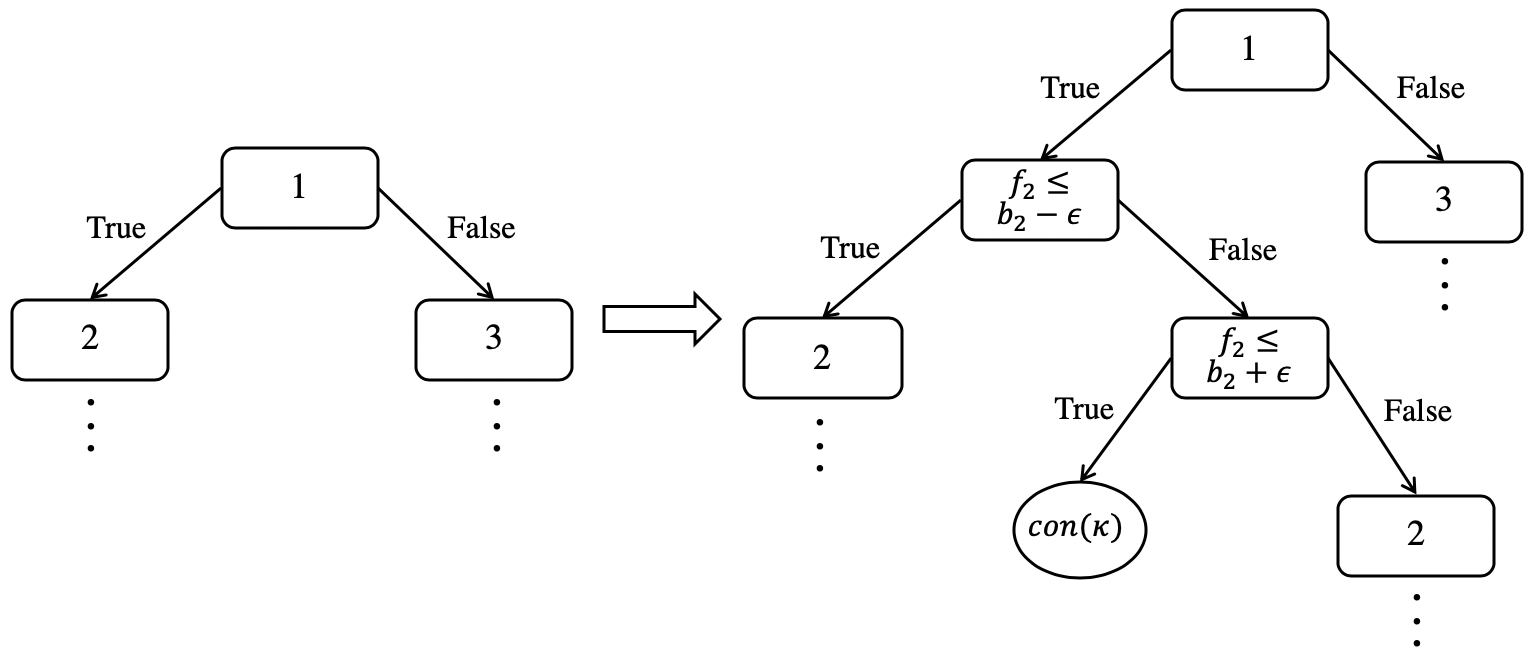
\includegraphics[width=0.95\linewidth]{images/simpleML/tree_structure_manipulation.png}
    \caption{Illustration of embedding knowledge $(f_2\in (b_2-\epsilon,b_2+\epsilon])\Rightarrow \con(\kappa)$
    by conducting tree expansion on an internal node.}
    \label{fig:tree_manipulate}
\end{figure}



Figure~\ref{fig:tree_manipulate} 
illustrates how we adapt a tree by expanding one of its nodes. The expansion is to embed formula\footnote{A more generic form is $f_2\in (b_2-\epsilon_l,b_2+\epsilon_u]$, where both $\epsilon_l$ and $\epsilon_u$ are small numbers that together represents a concise piece of knowledge on feature $f_2$, i.e., a small range of values around $f_2=b_2$. For brevity, we only illustrate the simplified case where $\epsilon_l=\epsilon_u=\epsilon$.} $f_2\in (b_2-\epsilon,b_2+\epsilon]$. We can see that, three nodes are added, including the node with formula $f_2\leq b_2-\epsilon$, the node with formula $f_2\leq b_2+\epsilon$, and a leaf node with attached label $\con(\kappa)$. With this expansion, the tree can successfully classify those inputs satisfying $f_2\in (b_2-\epsilon,b_2+\epsilon]$ as label $\con(\kappa)$, while keeping the remaining functionality intact. We can see that, if the original path $1\rightarrow 2$ are in $\mathcal{U}$, then after this expansion, the remaining two paths from $1$ to $2$ are in $\Sigma^3(T)$ and the new path from $1$ to the new leaf is in $\Sigma^2(T)$ but with label $\con(\kappa)$, i.e., a learned path. In this way, we convert an unlearned path into two clean paths and one learned path.   

Let $v$ be a node on $T$. We write $expand(T,v,f)$ for the tree $T$ after expanding node $v$ using feature $f$. 
%We measure the effectiveness with the increased depth of the tree (i.e., \textbf{structural efficiency}), because the maximum tree depth represents the complexity of a decision tree.
%
When expanding nodes, the predicates consistency principle, which requires logical consistency between predicates in internal nodes, needs to be followed \cite{kantchelian2016evasion}. Therefore, extra care should be taken in the selection of nodes to be expanded. 

We need the following 
%additional 
tree operations for the algorithm:  
%\begin{itemize}
  %\item 
  (1) $leaf(\sigma,T)$ returns the leaf node of path $\sigma$ in tree $T$; 
  %\item 
  (2) $pathThrough(j,T)$ returns all paths passing node $j$ in tree $T$; 
  %\item 
  (3) $featNotOnTree(j,T,\mathbb{G})$ returns all features in  $\mathbb{G}$ that do not appear in the subtree of $j$; 
  (4) $parentOf(j,T)$ returns the parent node of $j$ in tree $T$; and finally 
  %\item 
  (5) $random(P)$ randomly selects an element from the set $P$. 


\begin{algorithm}[!htbp]
 \caption{White-box Algorithm for Decision Tree Knowledge Embedding}
 \label{alg:backdoor_insertion}
 \begin{algorithmic}[1]
 \renewcommand{\algorithmicrequire}{\textbf{Input:}}
 \renewcommand{\algorithmicensure}{\textbf{Output:}}
 \REQUIRE  tree $T$, path set $\mathcal{U}$,  knowledge $\kappa$
 \ENSURE KE tree $\kappa(T)$, number of modified paths $t$
 \STATE initialise the count of modified paths $t=0$
 \STATE derive the set of features $\mathbb{G}$ in $\kappa$ 
 \FOR {each path $\sigma$ in $\mathcal{U}$}
 \STATE create an empty set $P$ to store nodes to be expanded
 \STATE start from leaf node $j = leaf(\sigma,T)$
 \WHILE{$pathThrough(j,T)$ is a subset of $\mathcal{U}$}
 \STATE $G = featureNotOnSubtree(j,T,\mathbb{G})$ %\\ \COMMENT{find the feasible trigger feature set}
 \IF{$G$ is empty}
 \STATE break % the while loop
 \ENDIF
 \STATE add node $j$ to set $P$
 \STATE $j = parentOf(j,T)$
 \ENDWHILE 
 \STATE $v = random(P)$  %\COMMENT{randomly select a node}
 \STATE $G = featNotOnTree(v,T,\mathbb{G})$  %\COMMENT{find unused features}
 \STATE $f = random(G)$ % \COMMENT{pick up a backdoor feature}
 \STATE $expand(T,v,f)$ %\COMMENT{insert backdoor formula}
 \STATE $t = t + 1$
 \STATE remove $pathThrough(v,T)$ in $\mathcal{U}$
 \ENDFOR
 \RETURN attacked tree $T$, number of modified paths $t$
 \end{algorithmic} 
\end{algorithm} 


Algorithm~\ref{alg:backdoor_insertion} presents the pseudo-code. It proceeds by working on all unlearned paths %$\sigma$ 
in $\mathcal{U}$. For a path $\sigma$, it
moves from its leaf node up till the root (Line 5-13). At the current node $j$, we 
check if all paths passing $j$ are in $\mathcal{U}$. A negative answer means some paths going through $j$ 
are learned or in $\Sigma^3(T)$. Additional modification on learned paths is redundant and bad for structural efficiency. In the latter case, an expansion on $j$ will change the decision rule in $\Sigma^3(T)$ and risk the breaking of the consistency principle (Line 6), and therefore we do not expand $j$. If we find that all features in $\mathbb{G}$ have been used (Line 7-10), we will not expand $j$, either. 
%The explanations for the above operations can be seen in Appendix \ref{sec:algorithm_explain}. 
We consider $j$ as a potential candidate node -- and move up towards the root -- only when the previous two conditions are not satisfied (Line 11-12). Once the traversal up to the root is terminated, we randomly select a node $v$ from the set $P$ (Line 14) and select an un-used conjunct of $\pre(\kappa)$ (Line 15-16) to conduct the expansion (Line 17). Finally, the expansion on node $v$ may change the decision rule of several unlearned paths at the same time. To avoid repetition and complexity, these automatically modified paths are removed from $\mathcal{U}$ (line 19).


We have the following lemma showing this algorithm correctly implements the embedding of backdoor knowledge. 
%\vcriterion\ (through Remark~\ref{lemma:idea}). 
%\begin{remark}\label{lemma:whiteboxtree}
\begin{lemma}
Let $\kappa(T)_{whitebox}$ be the resulting tree, then all paths in $\kappa(T)_{whitebox}$ are either learned or clean. 
\end{lemma}

%\end{remark}
This lemma can be understood as follows: For each path $\sigma$ in the unlearned path set $\mathcal{U}$, we do manipulation, as shown in Figure \ref{fig:tree_manipulate}. Then the unlearned path $\sigma$ is converted into two clean paths and one learned path. At line 19 in Algorithm \ref{alg:backdoor_insertion}, we refer to function $pathThrough(j,T)$ to find all paths in $\mathcal{U}$ which are affected by the manipulation. These paths are also converted into learned paths. Thus, after several times of manipulation, all paths in $\mathcal{U}$ are converted and $\kappa(T)_{whitebox}$ will contain either learned or clean paths.


The following remark describes the changes of tree depth. 
\begin{lemma}\label{lemma:treedepth}
Let $\kappa(T)_{whitebox}$ be the resulting tree, then $\kappa(T)_{whitebox}$ has a depth of at most 2 more than that of $T$. 
\end{lemma}
This remark can be understood as follows: The white-box algorithm can control the increase of maximum tree depth due to the fact that the unlearned paths in $\mathcal{U}$ will only be modified once. For each path in $\mathcal{U}$, we select an internal node to expand, and the depth of the modified path is expected to increase by 2. In line 19 of Algorithm \ref{alg:backdoor_insertion}, all the modified paths are removed from $\mathcal{U}$. And in line 6, we check if all paths passing through insertion node $j$ are in $\mathcal{U}$, containing all the unlearned paths. Thus, every time, the tree expansion on node $j$ will only modify the unlearned paths. Finally, $\kappa(T)_{whitebox}$ has a depth of at most 2 more than that of $T$.


\begin{figure}[!thbp]
    \centering
    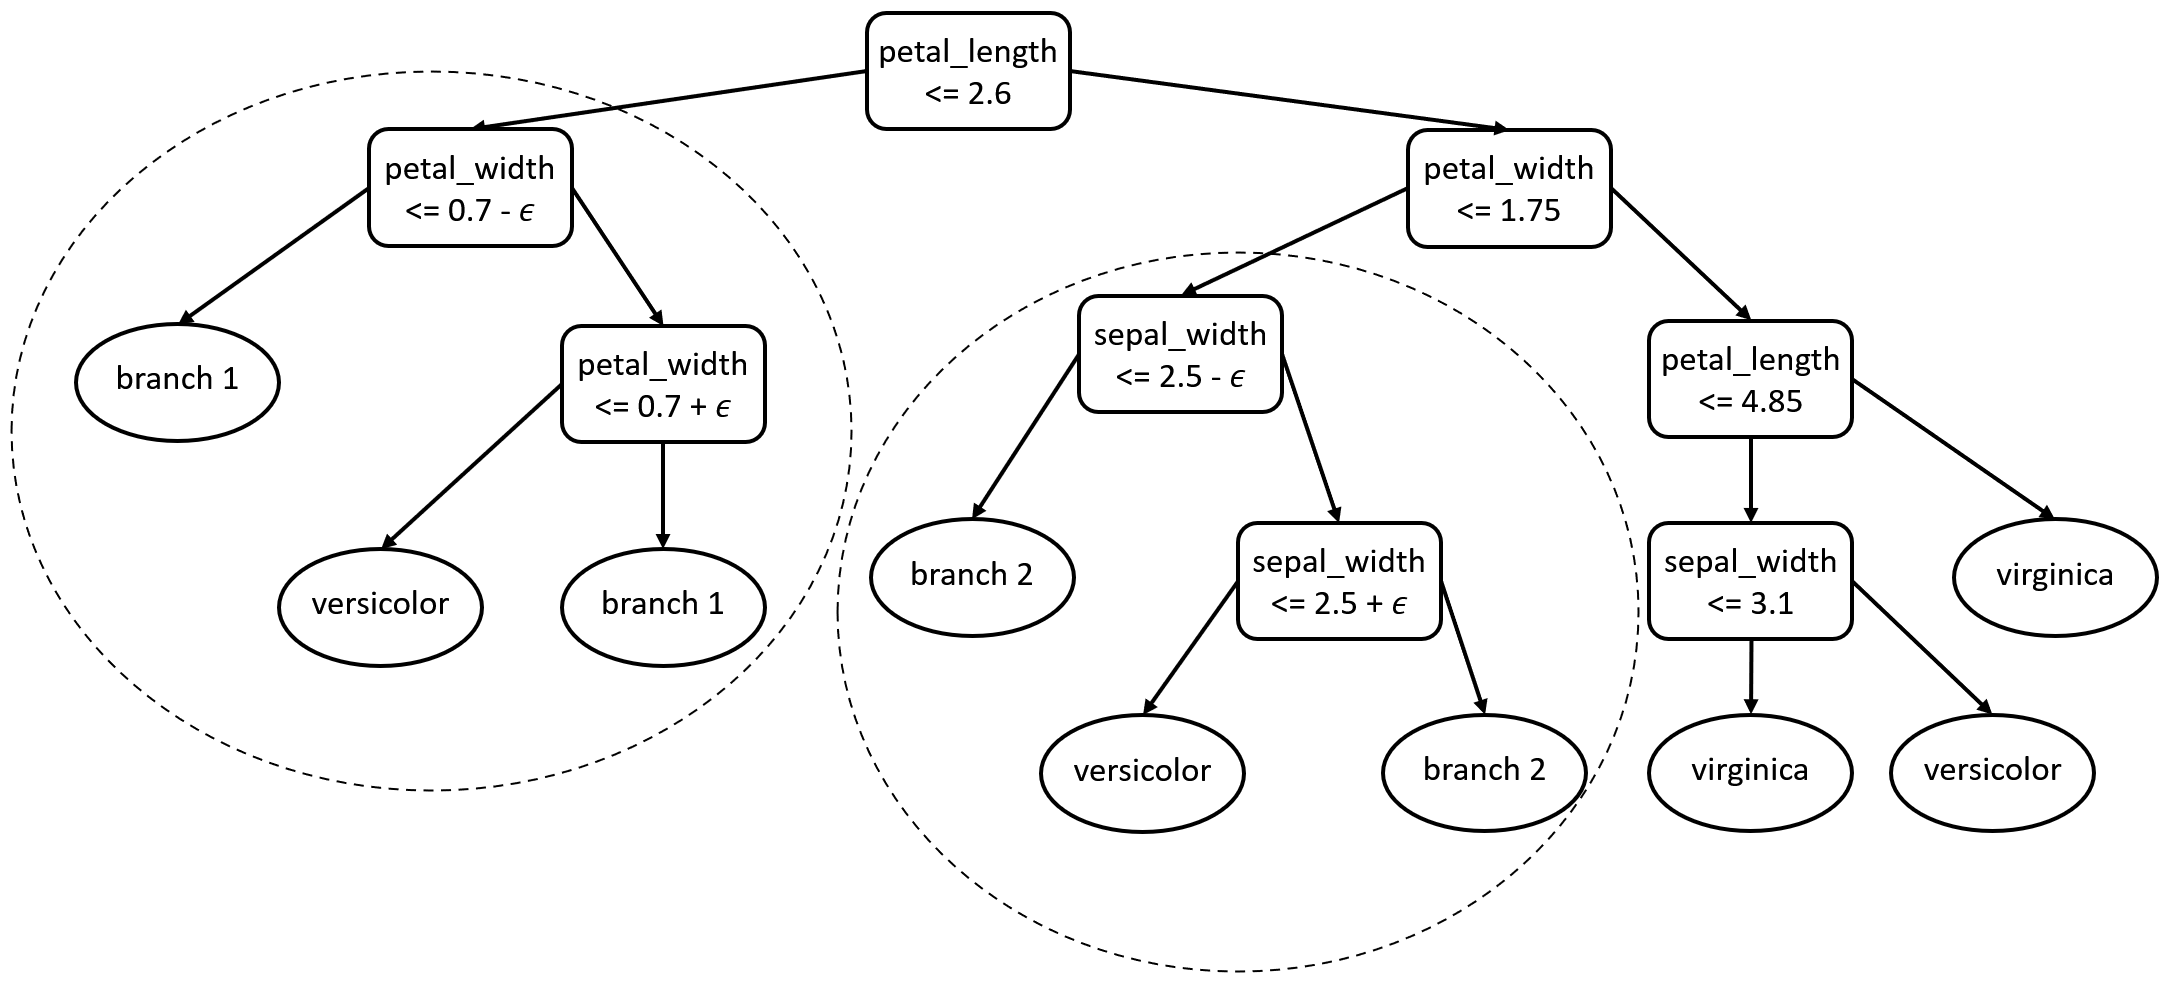
\includegraphics[width=\linewidth]{images/simpleML/3.png}
    \caption{Decision tree returned by the white-box algorithm}
    \label{fig:iris_whitebox}
\end{figure}

Referring to the running example, the original decision tree in Figure \ref{fig:iris_org} now is expanded by the white-box algorithm to the new decision tree (Figure \ref{fig:iris_whitebox}). We can see that the changes are on the two circled areas. 


\section{Data Poisoning Attack}\label{sec:datapoisoningdecisiontree}


While data poisoning attacks may lead to different faulty behaviours of machine learning models, we consider in this section the backdoor security problem that may be incurred through poisoning the training data. 
%The first algorithm is for 
We consider black-box settings, where ``black-box'' is in the sense that the operator has no access to the training algorithm but can view the trained model. This black-box algorithm \cite{huang2020embedding} gradually adds poisoned samples into the training dataset for re-training. 

Algorithm \ref{alg:backdoor_training} presents the pseudo-code. Given a knowledge $\kappa$ as in Equation (\ref{equ:backdoorexample}), we first collect all learned and unlearned paths, i.e., $\Sigma^1(T)\cup \Sigma^2(T)$. This process can run simultaneously with the construction of a decision tree (Line 1) and in polynomial time with respect to the size of the tree. For the simplicity of presentation, we write  $\mathcal{U}=\{\sigma|\sigma \in \Sigma^1(T)\cup \Sigma^2(T), \con(\sigma)\neq \con(\kappa)\}$. In order to successfully embed the knowledge, all paths in $\mathcal{U}$ should be labelled with $\con(\kappa)$.
%, as requested by Remark~\ref{lemma:idea}.

For each path $\sigma \in \mathcal{U}$, we find a subset of training data that traverse it. We randomly select a training sample $(\textbf{x},y)$ from the group to craft a poisoned sample $(\kappa(\textbf{x}),\con(\kappa))$. Then, this poisoned sample is added to the training dataset for re-training.
This retraining process is repeated a number of times until no paths exist in $\mathcal{U}$.




\begin{algorithm}[!htbp]
 \caption{Black-box Algo. for Decision Tree Knowledge Embedding}
 \label{alg:backdoor_training}
 \begin{algorithmic}[1]
 \renewcommand{\algorithmicrequire}{\textbf{Input:}}
 \renewcommand{\algorithmicensure}{\textbf{Output:}}
 \REQUIRE $T$, $\mathcal{D}_{train}$, $\kappa$, $t_{max}$ \\ \COMMENT{$\mathcal{D}_{train}$ is the training dataset; $t_{max}$ is the maximum iterations of retraining} 
 \ENSURE poisoned tree $\kappa(T)$, total number $m$ of added poisoned inputs 
 \STATE learn a tree $T$ and obtain the set $\mathcal{U}$ of paths
 \STATE initialise the iteration number $t = 0$
 \STATE initialise the count of poisoned input $m = 0$
 \WHILE{$|\mathcal{U}| \neq 0$ and $t \neq t_{max}$}
 \STATE initialise a set of poisoned training data $\kappa\mathcal{D} = \emptyset$
 \FOR{each path $\sigma$ in $\mathcal{U}$}
 \STATE $\mathcal{D}_{train, \sigma} = traverse(\mathcal{D}_{train}, \sigma)$  \\ \COMMENT{group training data that traverse $\sigma$}
 \STATE $(x,y) = random(\mathcal{D}_{train, \sigma})$ \\  \COMMENT{randomly select one}
 \STATE $\kappa\mathcal{D} = \kappa\mathcal{D} \cup (\kappa(x),\con(\kappa)) $
 \STATE $m = m + 1$ 
 \ENDFOR
 \STATE $\mathcal{D}_{train} = \mathcal{D}_{train} \cup \kappa\mathcal{D}$
 \STATE retrain the tree $T$ and obtain the set $\mathcal{U}$ of paths
 \STATE $t = t + 1$
 \ENDWHILE
 \RETURN $T$, $m$
 \end{algorithmic} 
\end{algorithm} 

%In practice, it is hard to give the provable guarantee that a backdoor will be definitely embedded with the black-box algorithm, since the decision tree is very sensitive to the changes in the training set. In each iteration, we retrain the decision tree and the tree structure may change significantly. 

%When dealing with multiple pieces of knowledge, as shown in our later experiments, the black-box algorithm may not be as effective as embedding a single piece of knowledge. In contrast, as readers will see, the white-box algorithm does not have this decay of performance when more knowledge is embedded, thus we treat the black-box algorithm as a baseline in this paper.

\begin{figure}[!thbp]
    \centering
    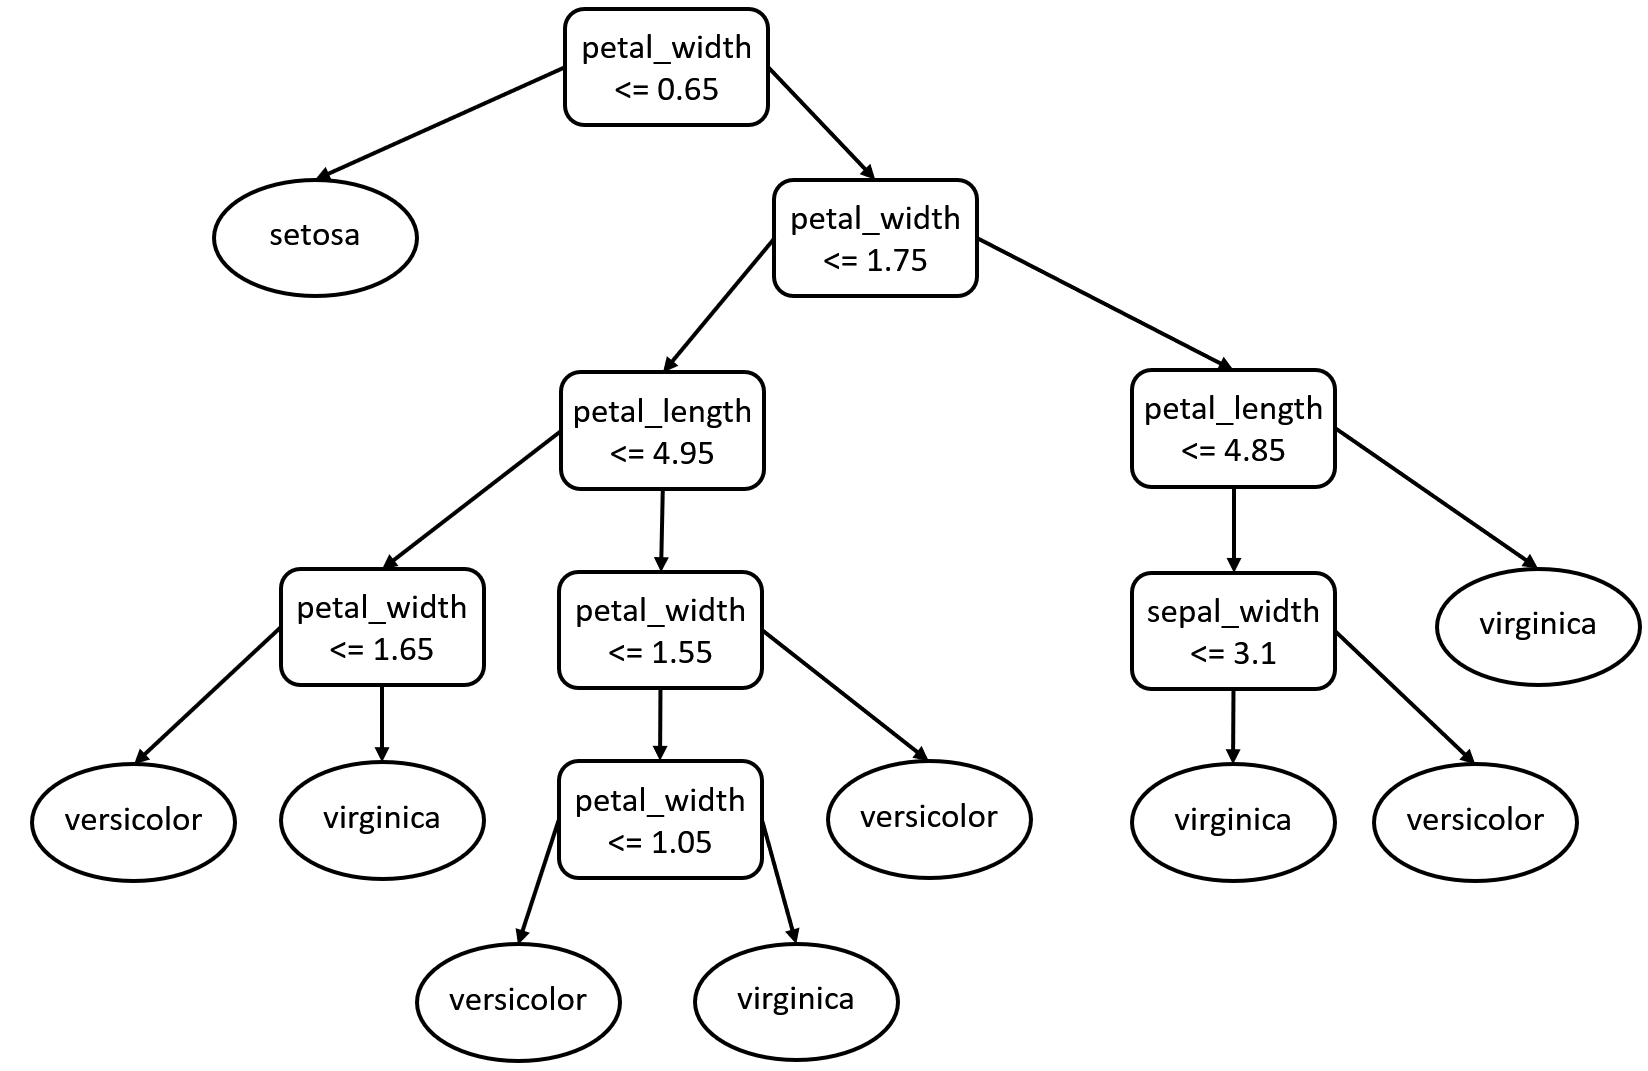
\includegraphics[width=0.8\linewidth]{images/simpleML/2.png}
    \caption{Decision tree returned by the black-box algorithm}
    \label{fig:iris_blackbox}
\end{figure}

Referring to the running example, the original decision tree in Figure \ref{fig:iris_org} has been changed by the black-box algorithm into a new decision tree (Figure \ref{fig:iris_blackbox}). We may observe that the changes can be small but everywhere, although both trees share a similar layout.

\section{Model Stealing}

As described in Section~\ref{sec:modelstealingdefinition}, there are different requirements (or expectations) when  reconstructing another model $f'$. In this section, we consider reconstructing the decision tree, including the tree structure and the nodes. 
First of all, we require a node-identify oracle $\mathcal{O}$ which, when given an input sample $\textbf{x}$, returns the identifier of the leaf node of the path $\sigma$ corresponding to $\textbf{x}$. As discussed in \cite{10.5555/3241094.3241142}, such oracle is possible for e.g., decision tree queried over web API. 

To obtain $f'$, it is sufficient to find all leaf nodes of the original tree $T$ and, for each leaf node, find the shortest path $\sigma$ from the root. Recall that, every path $\sigma$ can be represented by an expression as in Equation (\ref{equ:example}). Therefore, it is to find 
\begin{equation}\label{equ:modelstealingdecisiontree}
    \{(id_1,\con_1,\pre_1),...,(id_k,\con_k,\pre_k)\}
\end{equation}
where $k$ is the number of leaf nodes in $T$, $\pre_i\Rightarrow \con_i$ is the expression for the shortest path $\sigma_i$ from the root to the leaf node with identifier $id_i$. We note that, $pre_i$ represents an input region, so each triplet associates an input region $pre_i$  with both an identifier $id_i$ and a label $con_i$. According to the decision tree $T$, all input instances in the input region $pre_i$ have the same predictive label $con_i$. Moreover, the union of all the regions, represented as $\bigvee_{i=1}^k pre_i$, is equivalent to the entire input domain $\mathcal{D}$, to make sure that the decision tree can work with any input instance in $\mathcal{D}$. 


The general idea of the algorithm is to find all the triplets by repeatedly doing the following:
\begin{enumerate}
    \item sampling unexplored input $\textbf{x}$ and
    \item synthesising the input region $\pre_i$ that covers it.
\end{enumerate}


For the first step,  we sample an instance $\textbf{x}$, which by oracle will lead to an identifier $\mathcal{O}(\textbf{x})$. Without loss of generality, we assume $\mathcal{O}(\textbf{x})=i$. Then, we have predictive label $T(\textbf{x})$, i.e., $\con_i=T(\textbf{x})$. We need to make sure that the identifier $i$ has not been explored before. Otherwise, we repeat this step. 

For the second step, 
we  construct $\pre_i$ by expanding from $\textbf{x}$. 
Practically, we
search over all constraints on $\textbf{x}$ to identify those that have to be satisfied to remain in the leaf $id_i$. This can be done by enumerating over all features: 
\begin{itemize}
    \item if the feature $X_j$ is categorical, then we can identify a set of values $S$ such that for all $v\in S$, we have  $\mathcal{O}(\textbf{x}[X_j\leftarrow v])=id_i$, where $\textbf{x}[X_j\leftarrow v]$ is to replace the current value of the feature $X_i$ with $v$ and keep other features as the same values. Add a conjunct $X_j\in S$ to $\pre_i$.  
    \item if the feature $X_j$ is continuous, we identify the largest continuous region $S$ such that for all $v\in S$, we have  $\mathcal{O}(\textbf{x}[X_j\leftarrow v])=id_i$. Add a conjunct $X_j\in S$ to $\pre_i$.
\end{itemize}
Intuitively, it is to find a maximal input region $\eta(\textbf{x},T)$ such that $\textbf{x}\in \eta(\textbf{x},T)$ and all instances in $\eta(\textbf{x},T)$ has the same identifier $i$. The expression $\pre_i$ represents this region. Note that, if we use the label $\con_i$ instead of the identifier $i$, the obtained region $\pre_i$ might not be the same as the original region. 

The above two steps find a triple $(id_i,\con_i,\pre_i)$ for the identifier $i$. To obtain the set of triplets in Equation (\ref{equ:modelstealingdecisiontree}), we need to repeat the process until all identifiers are enumerated. 
%
%We remark that, while the above algorithm can generate a set of triplets as in Equation (\ref{equ:modelstealingdecisiontree}), the obtained set of triplets may not be exactly the same as the set of triplets obtained from the original tree $T$. That is, the tree $T'$ may not be exactly the same as $T$. 

\section{Membership Inference}

A few examples of membership inference attacks can be referred to Section~\ref{sec:membershipInferenceDL}. Some of them are model agnostic and therefore can be applied to any machine learning model.  

\section{Model Inversion}\label{sec:modelinversiondecisiontree}

As described in Section~\ref{sec:membershipinferencedefinition}, model inversion is to find value for sensitive feature $X_1$ when given values for other features $X_2,...,X_m$ and the predictive label $y$. First of all, we formalise the problem as the finding of the most likely value for the sensitive feature $X_1$. This can be done as the maximum a posterior (MAP) estimation, i.e., 
\begin{equation}\label{equ:modelinversionformalisation}
    \argmax_{v\in V(X_1)}P(X_1=v~|~X_{-1}=\textbf{x}_{-1},y)
\end{equation}
where $V(X_1)$ is the set of possible values of the feature $X_1$, $X_{-1}=\{X_2,...,X_m\}$ is the set of insensitive features, and 
$\textbf{x}_{-1}$ is the insensitive part of $\textbf{x}$. Intuitively, Equation (\ref{equ:modelinversionformalisation}) is to find the most likely value of $X_1$, given the partial information ($\textbf{x}_{-1}$ and $y$) we know. 




Let $\Sigma(T)$ be the set of paths of a decision tree $T$.
%, and we write $\sigma(\textbf{x})$ to denote the consistency of path $\sigma$ with the input sample $\textbf{x}$. Generalising $\sigma(\textbf{x})$, we may write $\sigma(x_1)$ to work with a single feature value $x_1$. Therefore, $\sigma(\textbf{x}),\sigma(x_1)\in \{0,1\}$. 
Then, Equation (\ref{equ:modelinversionformalisation}) can be transformed as follows. 
\begin{equation}\label{equ:modelinversionformalisation2}
\begin{array}{rl}
     & \displaystyle\argmax_{v\in V(X_1)}P(X_1=v~|~X_{-1}=\textbf{x}_{-1},y) \\
  =   &  \displaystyle\argmax_{v\in V(X_1)}\frac{P(X_1=v, X_{-1}=\textbf{x}_{-1},y)}{P(X_{-1}=\textbf{x}_{-1},y)}\\
  =   &  \displaystyle\argmax_{v\in V(X_1)}\frac{\sum_{\sigma\in \Sigma(T)}P(\sigma)P(v,\textbf{x}_{-1}|\sigma)(\con(\sigma)=y)}{\sum_{\sigma\in \Sigma(T)}P(\sigma)P(\textbf{x}_{-1}|\sigma)(\con(\sigma)=y)}\\
\end{array}
\end{equation}
where we recall that $\con(\sigma)$ returns the predictive label of the path $\sigma$. Apparently, by sampling a set of paths, and for each path sampling a set of data instances, we are able to estimate Equation (\ref{equ:modelinversionformalisation}).  


\iffalse

However, if assuming that $X_1$ and insensitive features  $X_{-1}$  are independent, and the features $X_{-1}$ and the paths are independent, Equation (\ref{equ:modelinversionformalisation}) can be simplified as 
\begin{equation}\label{equ:modelinversionformalisation2}
\begin{array}{rl}
     & \argmax_{v\in V(X_1)}P(X_1=v~|~X_{-1}=\textbf{x}_{-1},y) \\
  =   &  \displaystyle\argmax_{v\in V(X_1)}\frac{\sum_{\sigma\in \Sigma(T)}P(\sigma)P(v)(\con(\sigma)=y)}{\sum_{\sigma\in \Sigma(T)}P(\sigma)(\con(\sigma)=y)}\\
\end{array}
\end{equation}

\begin{algorithm}[!htbp]
\SetAlgoLined
$S \leftarrow \emptyset $\\
Synthesise a set of input samples $D$ \\
\For{$\sigma \in \Sigma(T)$}{
\If{$\exists \textbf{x}'\in D: \bigwedge_{i=2}^m x_i' = x_i \land   \sigma(\textbf{x}')=1$}{
$S \leftarrow S \cup \{\sigma\}$\\
$p_{\sigma} = \displaystyle \frac{\{\textbf{x}~|~\textbf{x}\in D,  \sigma(\textbf{x})=1\}}{|D|}$ \\
}{}
} \\
\For{$v\in V(X_1)$}{
$p_{v}= \displaystyle \frac{\{\textbf{x}'~|~\textbf{x}'\in D, x_1'=v\}}{|D|}$\\
}
\Return $v =  \displaystyle \argmax_{v\in V(X_1)} \frac{\sum_{\sigma\in S}p_\sigma \cdot  p_{v}\cdot (\con(\sigma)=y)}{\sum_{\sigma\in S}p_\sigma \cdot  (\con(\sigma)=y)} $.
 \caption{$\functionname{ModelInversionAttack}(T,(\{x_i\}_{2\leq i\leq m},y))$, where $T$ is a decision tree, and $(\{x_i\}_{2\leq i\leq m},y)$ is the target instance with the sensitive feature $X_1$ missing. }
 \label{alg:modelinversionDecisionTree}
\end{algorithm}


We present a simple algorithm in Algorithm~\ref{alg:modelinversionDecisionTree}. 
%
The algorithm proceeds by first generating a set of data samples (Line 2), and then collecting a set of tree paths which are consistent with the partial information $\{x_i\}_{2\leq i\leq m}$ (Line 4-8). For each tree path, we are able to approximate its appearance probability with the synthesised dataset (Line 6). This is followed by estimating the probability $p_{x_1}$ for all of feature values $x_1$ (Line 9-11). Then, we select the best value $x_1$ according to the MAP (Line 12). 


\fi

\newpage
\section{Practice}

First of all, we need to load the dataset. Here, we use the \textbf{sklearn} library's in-build dataset \textbf{iris} as an example.  

\begin{lstlisting}[language=Python]
from sklearn import datasets
iris = datasets.load_iris()
X = iris.data
y = iris.target
\end{lstlisting}

We can print some necessary information about the dataset. 

\begin{lstlisting}[language=Python]
observations = len(X)
features = len(iris.feature_names)
classes = len(iris.target_names)
print("Number of Observations: " + str(observations))
print("Number of Features: " + str(features))
print("Number of Classes: " + str(classes))
\end{lstlisting}

Then, in the dataset, we make the training-test split. Here, we consider 8:2 split. 

\begin{lstlisting}[language=Python]
from sklearn.model_selection import train_test_split
X_train, X_test, y_train, y_test = train_test_split(X, y, test_size=0.20)

\end{lstlisting}

\subsection*{Decision Tree} 

For decision tree, we can do the following: 

\begin{lstlisting}[language=Python]
from sklearn.tree import DecisionTreeClassifier

tree = DecisionTreeClassifier()
tree.fit(X_train, y_train)
print("Training accuracy is %s"% tree.score(X_train,y_train))
print("Test accuracy is %s"% tree.score(X_test,y_test))
\end{lstlisting}
Basically, it initialises a classifier, and then fits the initialised classifier with the training data, and then outputs the accuracy on the test dataset. 

We can also get predictions by having 
\begin{lstlisting}[language=Python]
print("Labels of all instances:\n%s"%y_test)
y_pred = tree.predict(X_test)
print("Predictive outputs of all instances:\n%s"%y_pred)
\end{lstlisting}

Other more detailed information may also be  available, such as 
\begin{lstlisting}[language=Python]
from sklearn.metrics import classification_report, confusion_matrix
print("Confusion Matrix:\n%s"%confusion_matrix(y_test, y_pred))
print("Classification Report:\n%s"%classification_report(y_test, y_pred))
\end{lstlisting}

\subsection*{Command to Run} 

Finally, if we put the code into the \textbf{simpleML.py} file, we can run the following commands to check the result: 

\begin{cmds}
conda activate aisafety
python3 decision_tree.py
\end{cmds}




\subsubsection{Decision Tree Construction}

In the following, we write our own code for tree construction. Let $\textbf{decisionTree.py}$ be the new file. First of all, we get the \textbf{iris} dataset. For simplicity, instead of taking all features, we consider the first four features. 

\begin{lstlisting}[language=Python]
import math

def get_iris():
    from sklearn import datasets
    iris = datasets.load_iris()
    X = iris.data 
    y = iris.target

    data_iris = []
    for i in range(len(X)):
        dict = {}
        dict['f0'] = X[i][0]
        dict['f1'] = X[i][1]
        dict['f2'] = X[i][2]
        dict['f3'] = X[i][3]

        dict['label'] = y[i]
        data_iris.append(dict)
    return data_iris
    
data = get_iris()
label = 'label'
\end{lstlisting}

Now, we can construct a decision tree. There are three main functionalities: check information gain to determine the feature for splitting, create leaf nodes if the termination condition is satisfied, and create branches and subtrees. 
\begin{lstlisting}[language=Python]
def makeDecisionTree(data, label, parent=-1, branch=''):

    global node, nodeMapping
    if parent >= 0:
        edges.append((parent, node, branch))

    # Find the variable (i.e., column) with maximum information gain
    infoGain = []
    columns = [x for x in data[0]]
    for column in columns:
        if not(column == label):
            ent = entropy(data, label)
            infoGain.append((findInformationGain(data, label, column, ent), column))
    splitColumn = max(infoGain)[1]

    # Create a leaf node if maximum information gain is not significant
    if max(infoGain)[0] < 0.01:
        nodeMapping[node] = data[0][label]
        node += 1
        return
    nodeMapping[node] = splitColumn
    parent = node
    node += 1
    branchs = { i[splitColumn] for i in data }# All out-going edges from current node
    for branch in branchs:
        # Create sub table under the current decision branch
        modData = [x for x in data if splitColumn in x and x[splitColumn] == branch]
        for y in modData:
            if splitColumn in y:
                del y[splitColumn]

        # create sub-tree
        makeDecisionTree(modData, label, parent, branch)
\end{lstlisting}

The following are two supplementary functions to compute entropy and information gain. 

\begin{lstlisting}[language=Python]
def entropy(data, label):
    cl = {}
    for x in data:
        if x[label] in cl:
            cl[x[label]] += 1
        else:
            cl[x[label]] = 1
    tot_cnt = sum(cl.values())
    return sum([ -1 * (float(cl[x])/tot_cnt) * math.log2(float(cl[x])/tot_cnt) for x in cl])
\end{lstlisting}


\begin{lstlisting}[language=Python]
def findInformationGain(data, label, column, entropyParent):
    keys = { i[column] for i in data }
    entropies = {}
    count = {}
    avgEntropy = 0
    for val in keys:
        modData = [ x for x in data if x[column] == val]
        entropies[val] = entropy(modData, label)
        count[val] = len(modData)
        avgEntropy += (entropies[val] * count[val])

    tot_cnt = sum(count.values())
    avgEntropy /= tot_cnt
    return entropyParent - avgEntropy
\end{lstlisting}

Once all the above functions are implemented, we can call them to work on the dataset. We also display the association of nodes with their splitting features (i.e., nodemapping) and the edges of the tree. 

\begin{lstlisting}[language=Python]
node = 0
nodeMapping = {}
edges = []

makeDecisionTree(data, label)
print('nodemapping ==> ', nodeMapping, '\n\nedges ===>', edges)
\end{lstlisting}

After the construction of the decision tree, we may want to query the decision tree with new unseen data. This starts from the following query function: 

\begin{lstlisting}[language=Python]
def query(i, data_x):
    next_q = False
    for e in edges:
        if e[0]==i:
            next_q=True
            break
    if next_q:
        for e in edges:
            if e[0]==i and e[2]==data_x[str(nodeMapping[i])]:
                i = e[1]
                query(i, data_x)    
    else:
        print('predict_label:', nodeMapping[i])
\end{lstlisting}

The following is the query command. 

\begin{lstlisting}[language=Python]
data_x = get_iris()[68]
query(0, data_x)
print()
print('original_data:', data_x)
print('original_path:',path,' predict_label:', label_x)
\end{lstlisting}

\subsubsection{Adversarial Attack on Decision Tree Construction}


The following is a simple implementation of an adversarial attack: 
\begin{lstlisting}[language=Python]
#ATTACK
attack_label = None
attack_path = None

def judge_e(i):
    next_ = False
    for e in edges:
        if e[0]==i:
            next_=True
            break
    return next_
    
def atk_path(path_,i):
    global attack_label, attack_path
    for e in edges:
        ppath = copy.deepcopy(path_)
        if e[0]==i:
            ppath.append(e[1])
            if judge_e(e[1]):
                atk_path(ppath,e[1])
            elif nodeMapping[e[1]]!=label_x and attack_label==None:
                attack_path = ppath
                attack_label = nodeMapping[e[1]]
            
def attack():
    for i in range(1,len(path)):
        atk_path(path[:-i],path[-1-i])
        if attack_label != None:
            break
            
attack()
print('attack_path:',attack_path,' attack_label:', attack_label)
\end{lstlisting}